\chapter{تصميم استراتيجيات التحكم (\LR{Control Strategies Design})}
\label{ch:control}

بعد إنجاز النمذجة الحركية والديناميكية الشاملة في الفصول السابقة، وامتلاك نموذج رياضي دقيق يصف سلوك روبوت (\LR{SCARA}) تحت تأثير الكتل المتغيرة والقوى الميكانيكية، ينتقل التركيز في هذا الفصل إلى تصميم استراتيجيات التحكم الآلي. الهدف الجوهري من نظام التحكم هو إجبار المفاصل الروبوتية على تتبع مسار مرجعي محدد مسبقاً بدقة عالية، مع ضمان استقرار النظام (\LR{Stability}) وامتلاكه للمتانة الكافية (\LR{Robustness}) لرفض الاضطرابات الخارجية والشكوك المعلمية المتمثلة في تغير كتلة الحمل المرفوع.

لتحقيق دراسة تحليلية وتطبيقية متكاملة، سيتم التدرج في هذا الفصل عبر ثلاث استراتيجيات تحكم رئيسية:
أولاً، سيتم تطبيق المتحكم التناسبية-التكاملية-التفاضلية (\LR{PID}) كخوارزمية تحكم خطية مستقلة تمثل المعيار المرجعي الصناعي. ثانياً، سيتم تصميم متحكم بالانزلاق (\LR{Sliding Mode Control - SMC}) لاخطي للتعامل مع التداخلات الديناميكية بين المفاصل. وأخيراً، سيتم اشتقاق وتصميم خوارزمية تحكم تكيفية متطورة تعتمد على العزم المحسوب ومصفوفة الانحدار (\LR{Regressor-based ACTC}) مع قانون تحديث مدعوم بتعديل سيغما (\LR{$\sigma$-modification})، لمنح الروبوت قدرة ذاتية على التكيف اللحظي مع الحمولات المجهولة.


\section{متحكم تناسبي-تكاملي-تفاضلي (\LR{PID Control})}
\label{sec:pid_control}

\subsection*{1. مبدأ الخوارزمية}
يُعد متحكم (\LR{PID}) خوارزمية تحكم خطية كلاسيكية تعتمد على الاستقلالية؛ حيث تعامل كل مفصل كنظام مستقل تماماً، وتتعامل مع التداخلات الديناميكية بين المفاصل وتغيرات الكتلة على أنها مجرد اضطرابات خارجية دون الحاجة لمعرفة النموذج الرياضي للنظام.

\subsection*{2. الشكل العام لقانون التحكم}
يُعطى قانون التحكم الكلاسيكي المستقل لكل مفصل بالصيغة الرياضية القياسية التالية:
\begin{equation}
u(t) = K_p e(t) + K_i \int_{0}^{t} e(\tau) d\tau + K_d \dot{e}(t)
\end{equation}
حيث $K_p, K_i, K_d$ تمثل أرباح التناسب، التكامل، والتفاضل على التوالي.

\subsection*{3. تهيئة النموذج وتعريف الأخطاء}
باعتبار الشعاع $q_{ref}$ يمثل المسار المرجعي المطلوب، والشعاع $q$ يمثل الموضع الفعلي للمفصل، يتم تعريف شعاع خطأ التتبع الموضعي $e$ وشعاع خطأ السرعة $\dot{e}$ لمفاصل الروبوت الثلاثة كما يلي:
\begin{equation}
e = \begin{bmatrix} \theta_{1ref} - \theta_1 \\ \theta_{2ref} - \theta_2 \\ d_{3ref} - d_3 \end{bmatrix} , \quad 
\dot{e} = \begin{bmatrix} \dot{\theta}_{1ref} - \dot{\theta}_1 \\ \dot{\theta}_{2ref} - \dot{\theta}_2 \\ \dot{d}_{3ref} - \dot{d}_3 \end{bmatrix}
\end{equation}

\subsection*{4. تطبيق الخوارزمية على النموذج}
يُصاغ شعاع إشارة التحكم الكلية $U_{PID}$ لجميع المفاصل بالشكل المصفوفي:
\begin{equation}
U_{PID} = K_P e + K_I \int e dt + K_D \dot{e}
\end{equation}
حيث $K_P, K_I, K_D$ هي مصفوفات قطرية تحوي أرباح التحكم لكل مفصل. بتعويض إشارة التحكم في النموذج الديناميكي الشامل للروبوت المستنتج في الفصل السابق، تصبح معادلة النظام المغلق:
\begin{equation}
\ddot{q} = \bar{M}^{-1} \left[ A \left( K_P e + K_I \int e dt + K_D \dot{e} \right) - R \dot{q} - D \right]
\end{equation}
\subsection{5. استجابة النظام عند قيم مختلفة للحمل ($m_L$)}
تم اختبار خوارزمية (\LR{PID}) عبر محاكاة تتبع إشارات مرجعية خطية (\LR{Step Response}) للمفاصل الثلاثة، حُددت بالقيم التالية: $\theta_{1ref} = 90^\circ$، $\theta_{2ref} = 90^\circ$، و $d_{3ref} = 0.2 \text{ m}$. يوضح الشكلان التاليان استجابة المفاصل عند تطبيق الخوارزمية باختبارين مختلفين لكتلة الحمل المرفوع ($m_L$):

\begin{figure}[H]
    \centering
    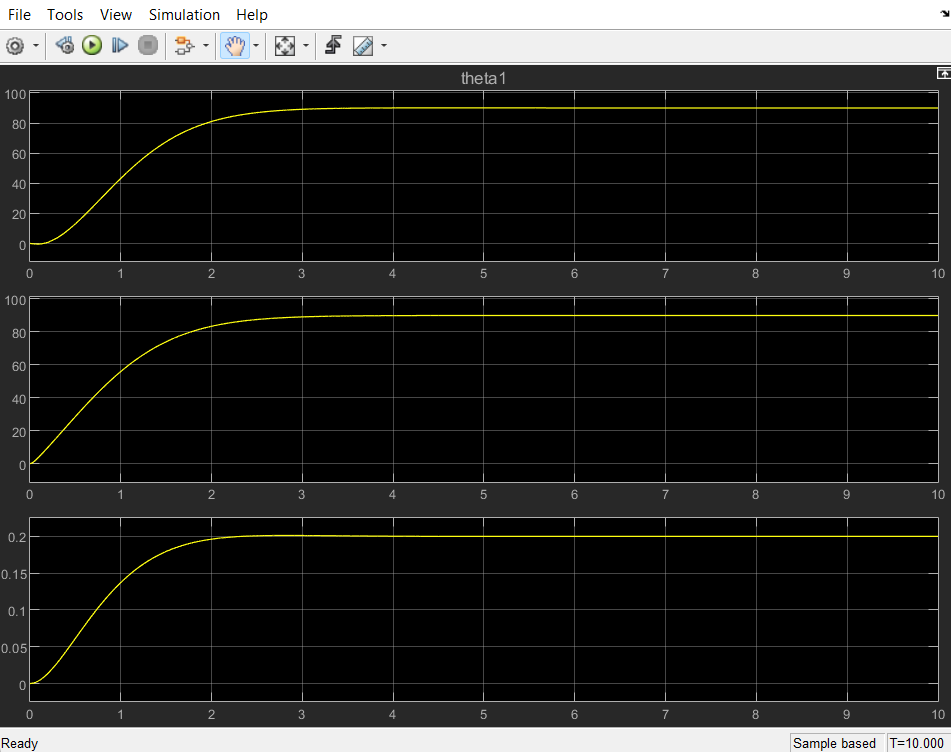
\includegraphics[width=0.8\textwidth]{resources/images/PID_res_m0.png}
    \caption{\centering{استجابة متحكم \LR{PID} بدون حمل ($m_L = 0 \text{ kg}$)}}
    \label{fig:pid_m0}
\end{figure}
  

\begin{figure}[H]
    \centering
    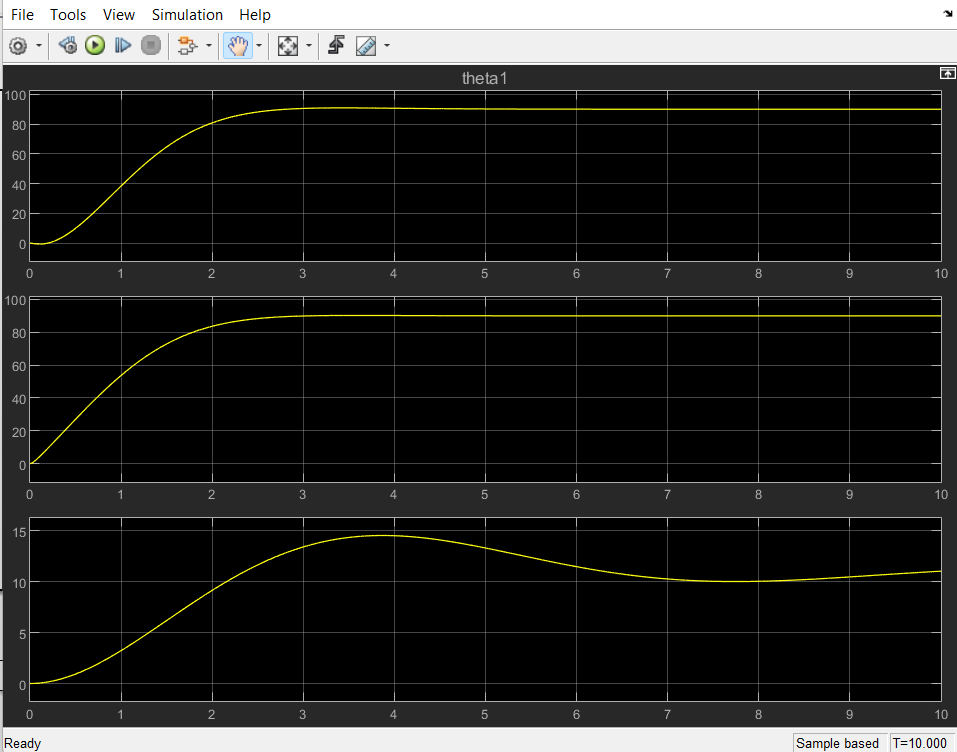
\includegraphics[width=0.8\textwidth]{resources/images/PID_res_m10.png}
    \caption{\centering{استجابة متحكم \LR{PID} عند إضافة حمل ($m_L = 10 \text{ kg}$)}}
    \label{fig:pid_m10}
\end{figure}

يُلاحظ من الشكل (\ref{fig:pid_m0}) أن المتحكم في حالة اللاحمل ($m_L = 0$) قادر على توجيه المفاصل نحو القيم المرجعية بدقة واستقرار تام وبدون خطأ حالة مستقرة. 

في المقابل، عند إضافة حمل كتلته ($10 \text{ kg}$) كما في الشكل (\ref{fig:pid_m10})، يتدهور أداء المتحكم الكلاسيكي بشكل حاد. يظهر هذا الانهيار بوضوح شديد في المفصل الانسحابي ($d_3$)، حيث ينحرف المسار الفعلي بشكل كارثي مبتعداً عن القيمة المرجعية ($0.2$) ليصل إلى قيم تفوق ($14$). يعود هذا الفشل إلى عجز أرباح الـ (\LR{PID}) الثابتة عن توليد إشارة تحكم كافية لتعويض الزيادة الضخمة في قوى الجاذبية وعزوم القصور الذاتي الناتجة عن الحمل الجديد، مما يثبت افتقار هذه الخوارزمية للمتانة (\LR{Robustness}) المطلوبة في التطبيقات الصناعية متغيرة الأوزان.
\section{التحكم بالانزلاق (\LR{Sliding Mode Control - SMC})}
\label{sec:smc_control}

\subsection*{1. مبدأ الخوارزمية}
تُصنف خوارزمية التحكم بالانزلاق (\LR{SMC}) كواحدة من أقوى استراتيجيات التحكم اللاخطي المتين (\LR{Robust Control}). تعتمد الفكرة الأساسية على إجبار مسار النظام الديناميكي للوصول إلى سطح رياضي مصمم مسبقاً يُدعى "سطح الانزلاق" (\LR{Sliding Surface})، ثم إبقائه مقيداً على هذا السطح. يوفر هذا الأسلوب مناعة عالية جداً ضد التغيرات المعلمية (مثل تغير كتلة الحمل) والاضطرابات الخارجية.

\subsection*{2. الشكل العام لقانون التحكم}
يتكون قانون التحكم بالانزلاق من مركبين أساسيين:
\begin{equation}
u(t) = u_{eq}(t) + u_{sw}(t)
\end{equation}
حيث:
\begin{itemize}
    \item $u_{eq}$: قانون التحكم المكافئ (\LR{Equivalent Control})، وظيفته إبقاء النظام على السطح بافتراض عدم وجود اضطرابات (يعتمد على النموذج الاسمي).
    \item $u_{sw}$: قانون التبديل (\LR{Switching Control})، وظيفته التغلب على الشكوك ودفع النظام نحو السطح في حال انحرافه عنه.
\end{itemize}

\subsection*{3. تهيئة النموذج وتعريف الأخطاء}
باستخدام نفس تعريفات الخطأ الموضعي $e = q_{ref} - q$ وخطأ السرعة $\dot{e} = \dot{q}_{ref} - \dot{q}$، يتم تعريف شعاع سطح الانزلاق $S$ بأبعاد $3 \times 1$ لمفاصل الروبوت بالمعادلة:
\begin{equation}
S = \dot{e} + \Lambda e
\end{equation}
حيث $\Lambda$ مصفوفة قطرية موجبة تماماً تحدد ميل سطح الانزلاق وسرعة تقارب الخطأ نحو الصفر. 
بأخذ المشتق الزمني لسطح الانزلاق نحصل على:
\begin{equation}
\dot{S} = \ddot{e} + \Lambda \dot{e} = \ddot{q}_{ref} - \ddot{q} + \Lambda \dot{e}
\end{equation}

\subsection*{4. تطبيق الخوارزمية على النموذج}
بالاعتماد على النموذج الديناميكي الشامل للروبوت المستنتج في الفصل السابق: $\ddot{q} = \bar{M}^{-1} [A u - R \dot{q} - D]$، نقوم بتعويض $\ddot{q}$ في معادلة $\dot{S}$:
\begin{equation}
\dot{S} = \ddot{q}_{ref} - \bar{M}^{-1} [A u - R \dot{q} - D] + \Lambda \dot{e}
\end{equation}
لإيجاد التحكم المكافئ $u_{eq}$، نضع $\dot{S} = 0$، فنحصل على:
\begin{equation}
u_{eq} = A^{-1} \left[ \bar{M} (\ddot{q}_{ref} + \Lambda \dot{e}) + R \dot{q} + D \right]
\end{equation}
لضمان شرط الوصول لسطح الانزلاق (\LR{Reachability Condition}) في ظل وجود تغير في الكتلة، نضيف حد التبديل باختيار $u_{sw} = A^{-1} \bar{M} K \text{sgn}(S)$، حيث $K$ مصفوفة أرباح التبديل القطرية. ليصبح قانون التحكم النهائي المطبق على المحركات:
\begin{equation}
u_{SMC} = A^{-1} \left[ \bar{M} (\ddot{q}_{ref} + \Lambda \dot{e}) + R \dot{q} + D + K \text{sgn}(S) \right]
\end{equation}

\subsection{5. استجابة النظام عند قيم مختلفة للحمل ($m_L$)}
تم اختبار خوارزمية (\LR{SMC}) على نفس المسارات المرجعية السابقة ($\theta_{1ref} = \theta_{2ref} = 90^\circ$ و $d_{3ref} = 0.2 \text{ m}$). توضح الأشكال التالية متانة المتحكم عند تغير الحمل:


 \begin{figure}[H]
     \centering
     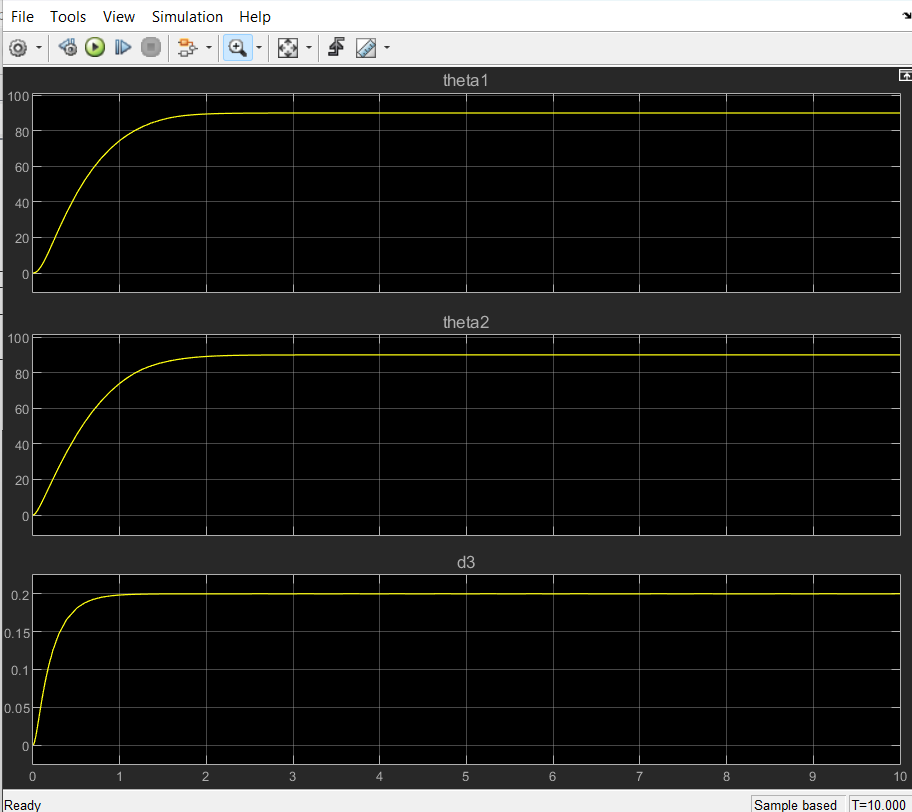
\includegraphics[width=0.8\textwidth]{resources/images/SMC_res_m0.png}
     \caption{\centering{استجابة متحكم \LR{SMC} بدون حمل ($m_L = 0 \text{ kg}$)}}
     \label{fig:smc_m0}
 \end{figure}

 \begin{figure}[H]
     \centering
     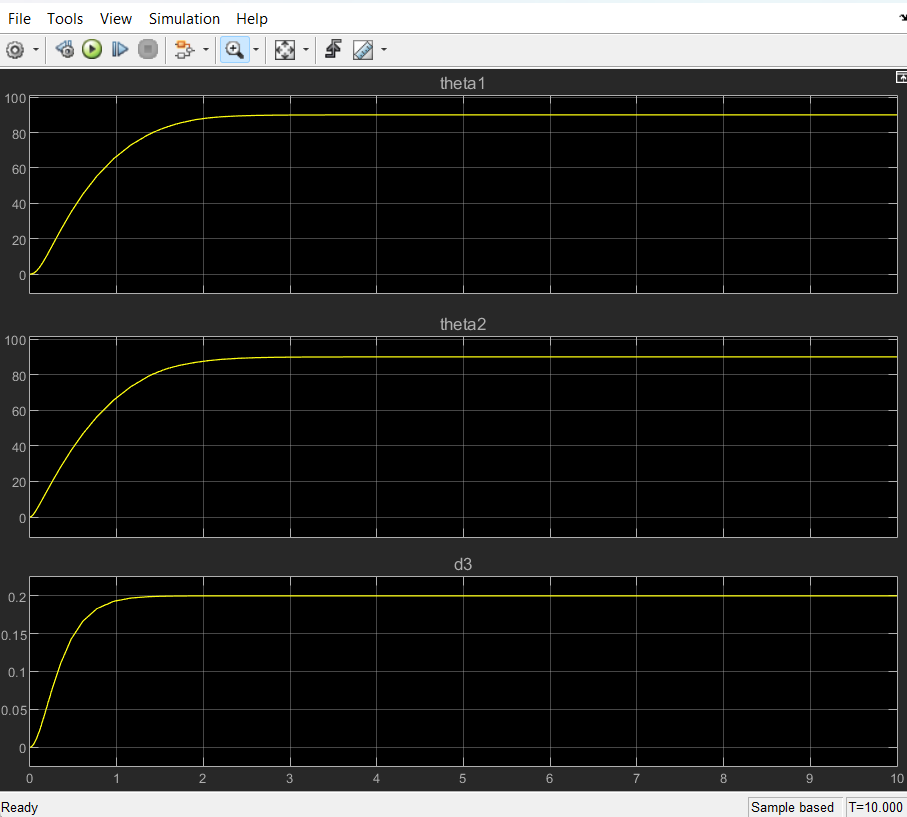
\includegraphics[width=0.8\textwidth]{resources/images/SMC_res_m10.png}
     \caption{\centering{استجابة متحكم \LR{SMC} عند إضافة حمل ($m_L = 10 \text{ kg}$)}}
     \label{fig:smc_m10}
 \end{figure}

على عكس الانهيار الذي حدث في خوارزمية (\LR{PID})، يُلاحظ من المنحنيات أن متحكم (\LR{SMC}) حافظ على دقة تتبع عالية للمسار المرجعي واستقرار ممتاز في المفصل الانسحابي حتى عند إضافة الحمل الأقصى ($10 kg$)، حيث استغرق النظام زمناً يقارب ($1 sec$) ليصل إلى حالة الاستقرار التام. يعود هذا الأداء المتين إلى تأثير حد التبديل اللاخطي الذي يجبر النظام على البقاء ضمن سطح الانزلاق المنيع ضد الاضطرابات الخارجية وتغيرات القصور الذاتي.
\section{التحكم التكيفي المعتمد على العزم المحسوب (\LR{Adaptive Computed Torque Control})}
\label{sec:actc_control}

\subsection*{1. مبدأ الخوارزمية}
تدمج هذه الخوارزمية بين تقنية الإلغاء الخطي للديناميكية (\LR{Feedback Linearization}) وبين آلية تكيفية مستمرة لتحديث معلمات النظام المجهولة (مثل كتلة الحمل وعزوم القصور الذاتي) في الزمن الفعلي. يتم استبدال الثوابت الفيزيائية المجهولة بمعلمات مُقَدَّرَة تتحدث قيمتها بناءً على خطأ التتبع، مما يوفر أداءً ناعماً ومستقراً دون الحاجة لإشارات التبديل القاسية.

\subsection*{2. الشكل العام لقانون التحكم ومبدأ الانحدار}
تعتمد الخوارزمية على خاصية خطية المعلمات (\LR{Linearity in Parameters})، حيث يمكن فصل النموذج الديناميكي إلى مصفوفة انحدار (\LR{Regressor} $Y$) تحوي المتغيرات الحركية المعروفة، وشعاع معلمات ($\Theta$) يحوي الثوابت المجهولة. 

لتطبيق الخوارزمية بشكل عملي ومستقل لكل مفصل، يُكتب قانون التحكم التكيفي للمفصل $(i)$ بالصيغة القياسية التالية:
\begin{equation}
\tau_i = \hat{\theta}_i^T Y_i - K_{s,i} s_i
\label{eq:adaptive_general_i}
\end{equation}
حيث $\hat{\theta}_i$ هو شعاع المعلمات المُقَدَّرَة للمفصل، و $Y_i$ شعاع الانحدار الخاص به، و $s_i$ هو سطح الانزلاق، و $K_{s,i}$ ربح تحكم موجب لضمان تقارب الخطأ.

\subsection*{3. تفكيك النموذج وتعريف المعلمات المُقَدَّرَة}
بتفصيل المعادلة (\ref{eq:adaptive_general_i}) بناءً على القوى الفيزيائية المؤثرة على المفصل (عطالة، احتكاك، جاذبية)، يأخذ قانون التحكم شكله التفصيلي المطبق على المحركات كما يلي:
\begin{equation}
\tau_i = \hat{\theta}_{M,i} (M_e(q)\ddot{q}_r)_i + \hat{\theta}_{V,i} (K_v \dot{q})_i + \hat{\theta}_{G,i} G_i(q) + \hat{\theta}_{0,i} - K_{s,i} s_i
\label{eq:adaptive_detailed_i}
\end{equation}

حيث تم تخصيص معامل مُقَدَّر منفصل لكل مركب ديناميكي:
\begin{itemize}
    \item $\hat{\theta}_{M,i}$: المُعامل التكيفي المُقَدَّر لتعويض تغيرات عزم القصور الذاتي الكلي (والذي يتأثر بشدة بتغير كتلة الحمل $m_L$).
    \item $\hat{\theta}_{V,i}$: المُعامل المُقَدَّر لتعويض قوى الاحتكاك اللزج والقوى المرتبطة بالسرعة.
    \item $\hat{\theta}_{G,i}$: المُعامل المُقَدَّر لتعويض عزوم الجاذبية الأرضية.
    \item $\hat{\theta}_{0,i}$: المُعامل المُقَدَّر لتعويض الاحتكاك السكوني (\LR{Coulomb Friction}) والاضطرابات الثابتة المجهولة.
\end{itemize}

\subsection*{4. تعريف الأخطاء وقانون التحديث (\LR{Adaptation Law})}
يتم تعريف سطح الانزلاق للمفصل $(i)$ بالاعتماد على خطأ التتبع الموضعي $e_i = q_i - q_{ref,i}$ كالتالي:
\begin{equation}
s_i = \dot{e}_i + \lambda_i e_i
\end{equation}
حيث $\lambda_i$ ثابت إيجابي يحدد ميل السطح. ولتحديث المعلمات المُقَدَّرَة $\hat{\theta}_i$ لحظياً وبشكل يضمن استقرار النظام وفق نظرية ليابونوف، يتم تطبيق قانون التحديث التفاضلي المدعوم بتعديل سيغما (\LR{$\sigma$-modification}) لمنع انحراف القيم:
\begin{equation}
\dot{\hat{\theta}}_i = \Gamma_i Y_i^T s_i - \Gamma_i \sigma_i \hat{\theta}_i
\end{equation}
حيث $\Gamma_i$ مصفوفة أرباح التعلم اللحظي، و $\sigma_i$ عامل تخميد إيجابي صغير.
\subsection*{5. استجابة النظام عند قيم مختلفة للحمل ($m_L$)}
تم اختبار خوارزمية (\LR{ACTC}) لمحاكاة تتبع المسارات المرجعية ($\theta_{1ref} = \theta_{2ref} = 90^\circ$ و $d_{3ref} = 0.2 \text{ m}$) مع تغيير ظروف التحميل للتحقق من قدرة الخوارزمية على التكيف الذاتي:


 \begin{figure}[H]
     \centering
     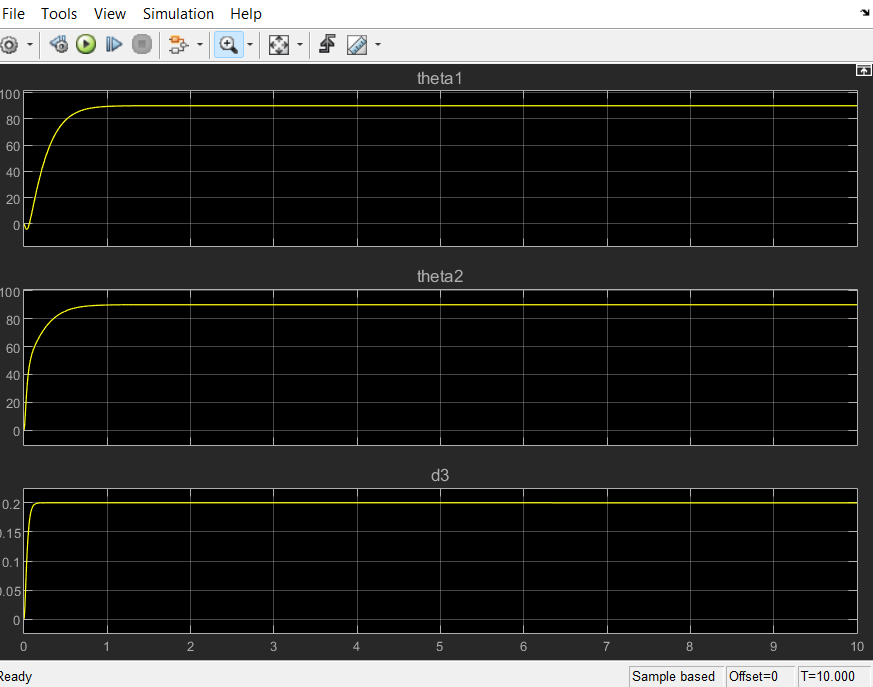
\includegraphics[width=0.8\textwidth]{resources/images/ACTC_res_m0.png}
     \caption{\centering{استجابة متحكم \LR{ACTC} وتتبع المسار بدون حمل ($m_L = 0 \text{ kg}$)}}
     \label{fig:actc_m0}
 \end{figure}

 \begin{figure}[H]
     \centering
     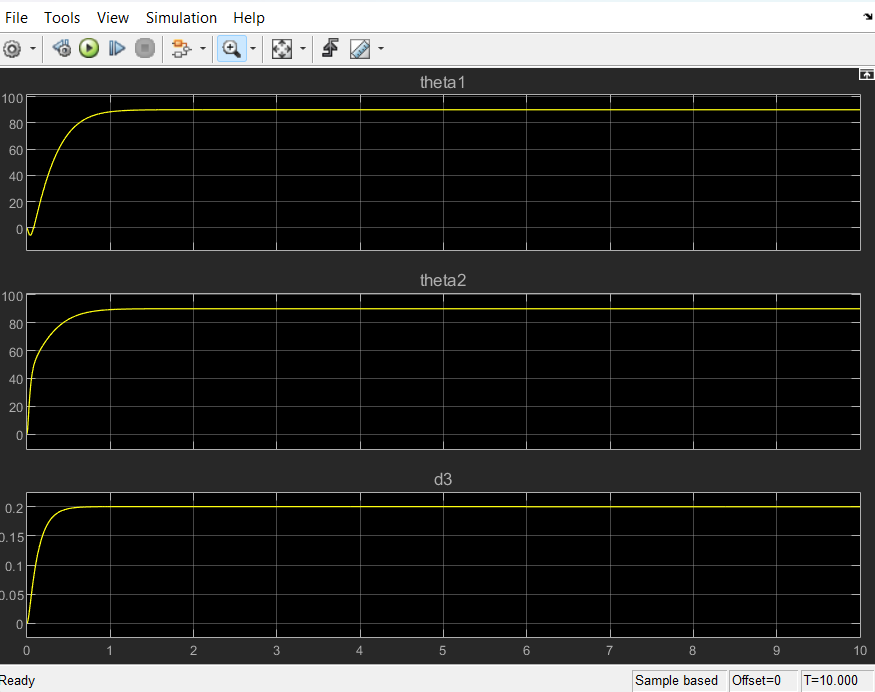
\includegraphics[width=0.8\textwidth]{resources/images/ACTC_res_m10.png}
     \caption{\centering{استجابة متحكم \LR{ACTC} وتحديث المعلمات لحظياً عند إضافة حمل ($m_L = 10 \text{ kg}$)}}
     \label{fig:actc_m10}
 \end{figure}

يُلاحظ من المنحنيات ظهور انحراف أولي سالب (\LR{Initial Undershoot}) لفترة وجيزة جداً في استجابة المفصل الأول ($\theta_1$) قبل انطلاقه نحو القيمة المرجعية. هذا الانحراف يعكس الطبيعة الفيزيائية الدقيقة للمحاكاة والتداخل الديناميكي (\LR{Dynamic Coupling}) بين المفاصل؛ فالتسارع الابتدائي العنيف للمفصل الثاني لتتبع المسار يولد عزم رد فعل يؤثر عكسياً على المفصل الأول، وسرعان ما تقوم خوارزمية (\LR{ACTC}) بتدارك هذا الاضطراب اللحظي وتصحيح المسار بقوة ونعومة.

بشكل عام، تظهر النتائج تفوقاً ديناميكياً وهندسياً واضحاً للمتحكم التكيفي. في حالة اللاحمل ($m_L = 0$)، استجاب النظام بسرعة فائقة محققاً زمن استقرار (\LR{Settling Time}) يقارب ($0.1 \text{ s}$). أما عند إضافة الحمل الأقصى المفاجئ ($10 \text{ kg}$)، فبدلاً من الانهيار كما في (\LR{PID}) أو استهلاك طاقة تبديل قاسية كما في (\LR{SMC})، قامت الآلية التكيفية بتقدير الزيادة اللحظية في القصور الذاتي وتحديث المعامل $\hat{\theta}_{M,3}$ داخلياً، ليتمكن النظام من استعادة استقراره التام خلال زمن قياسي لم يتجاوز ($0.5 \text{ s}$). نتج عن ذلك تتبع مسار عالي الدقة، وإشارات تحكم ناعمة خالية من ظاهرة الاهتزاز (\LR{Chattering})، مما يجعله الحل الأمثل صناعياً.
\section{مقارنة استراتيجيات التحكم واختيار الخوارزمية الأمثل}
\label{sec:control_comparison}

بعد التطبيق والتحليل المعمق لخوارزميات التحكم الثلاث (\LR{PID}، \LR{SMC}، و \LR{ACTC}) على النموذج الديناميكي الشامل لروبوت (\LR{SCARA})، واختبارها تحت ظروف تحميل متغيرة (من حالة اللاحمل إلى حمل أقصى $m_L = 10 \text{ kg}$)، يمكن تلخيص الفروقات الجوهرية بين هذه الاستراتيجيات من حيث الأداء الديناميكي، المتانة، والعبء الحسابي في الجدول التالي:
\begin{table}[H]
    \centering
    \caption{مقارنة هندسية بين استراتيجيات التحكم المطبقة على الروبوت}
    \label{tab:control_comparison}
    % إضافة تعليمات إيقاف المط (raggedright) والتوسيط (centering) للأعمدة
    \begin{tabular}{|>{\centering\arraybackslash}p{0.14\linewidth}|>{\raggedright\arraybackslash}p{0.21\linewidth}|>{\raggedright\arraybackslash}p{0.22\linewidth}|>{\raggedright\arraybackslash}p{0.21\linewidth}|>{\centering\arraybackslash}p{0.12\linewidth}|}
        \hline
        \textbf{الخوارزمية} & \textbf{دقة التتبع الموضعي} & \textbf{المتانة ضد تغيرات الحمل ($m_L$)} & \textbf{زمن الاستقرار} & \textbf{التعقيد الحسابي برمجياً} \\
        \hline
        \textbf{الكلاسيكي (\LR{PID})} & ممتازة في حالة اللاحمل، وضعيفة عند السرعات العالية. & منهارة (تأثر شديد بزيادة عزم القصور الذاتي للوصلة). & سريع في اللاحمل، وينهار (يفقد الاستقرار) عند إضافة الحمل. & بسيط جداً (لا يتطلب نموذج رياضي). \\
        \hline
        \textbf{الانزلاقي (\LR{SMC})} & عالية جداً. & ممتازة (مناعة تامة ضد الاضطرابات الخارجية). & \centering{جيد} & متوسط (يتطلب معرفة النموذج الاسمي). \\
        \hline
        \textbf{التكيفي (\LR{ACTC})} & عالية جداً. & ممتازة (تكيف ذاتي وتقدير لحظي ). & \centering{قياسي وسريع } & عالي (يتطلب تفكيك وحساب مصفوفة الانحدار $Y$). \\
        \hline
    \end{tabular}
\end{table}

\subsection*{القرار الهندسي: اعتماد خوارزمية (\LR{ACTC})}
بناءً على المعطيات التحليلية السابقة وطبيعة المهمة الصناعية لروبوت (\LR{SCARA}) المدروس (والتي تتمثل في نقل حمولات متغيرة الوزن بسرعات عالية)، \textbf{تم اختيار خوارزمية التحكم التكيفي المعتمد على العزم المحسوب (\LR{ACTC})} لتكون الاستراتيجية النهائية والمعتمدة في هذا المشروع. 

يأتي هذا الاختيار مبرراً بالنقاط والمزايا الهندسية التالية:
\begin{enumerate}
    \item \textbf{زمن استجابة قياسي:} أثبتت الخوارزمية قدرتها على استعادة استقرار النظام وتصفير خطأ التتبع خلال زمن قصير جداً ($0.5 \text{ s}$) حتى عند تعرض الروبوت  لصدمة تحميل ($10 \text{ kg}$)، مع امتصاص ذكي لعزوم التداخل الديناميكي بين المفاصل.
    \item \textbf{الاستغناء عن المعايرة اليدوية:} قدرة المتحكم التلقائية على تقدير الزيادة في القصور الذاتي وتحديث المعاملات المجهولة (مثل $\hat{\theta}_{M,3}$) لحظياً، مما يغني عن الحاجة لإعادة ضبط أرباح التحكم يدوياً عند كل تغيير في وزن القطعة المنقولة.
    \item \textbf{الحفاظ على العمر الافتراضي للمحركات:} على عكس متحكم (\LR{SMC}) الذي يضمن المتانة على حساب إرهاق المحركات بجهود تبديلية عالية التردد (\LR{Chattering})، توفر خوارزمية (\LR{ACTC}) إشارات تحكم ناعمة ومستمرة خالية من الاهتزازات، مما يقلل من التآكل الميكانيكي في المفاصل والارتفاع الحراري في ملفات المحركات.
\end{enumerate}

بهذا الاستنتاج، نكون قد أتممنا تصميم واختبار "العقل" البرمجي القادر على قيادة ذراع الروبوت بكفاءة صناعية عالية.